\section{Marco teórico}

\subsection{Eje lineal}
Los ejes lineales se componen de 2 elementos mecánicos, un riel o guía y un rodamiento, se utilizan en aplicaciones de movimiento lineal de precisión como mesas posicionadoras o para reducir la fricción en el transporte de algún material. La guía puede tener un perfil circular o cuadrado con formas de T o I, y son fabricados con un proceso de rectificado para ajustar las tolerancias adecuadas y asegurar una superficie con fricción constante de modo que el rodamiento tenga un movimiento fluido en toda la trayectoria.\\
\begin{center}
    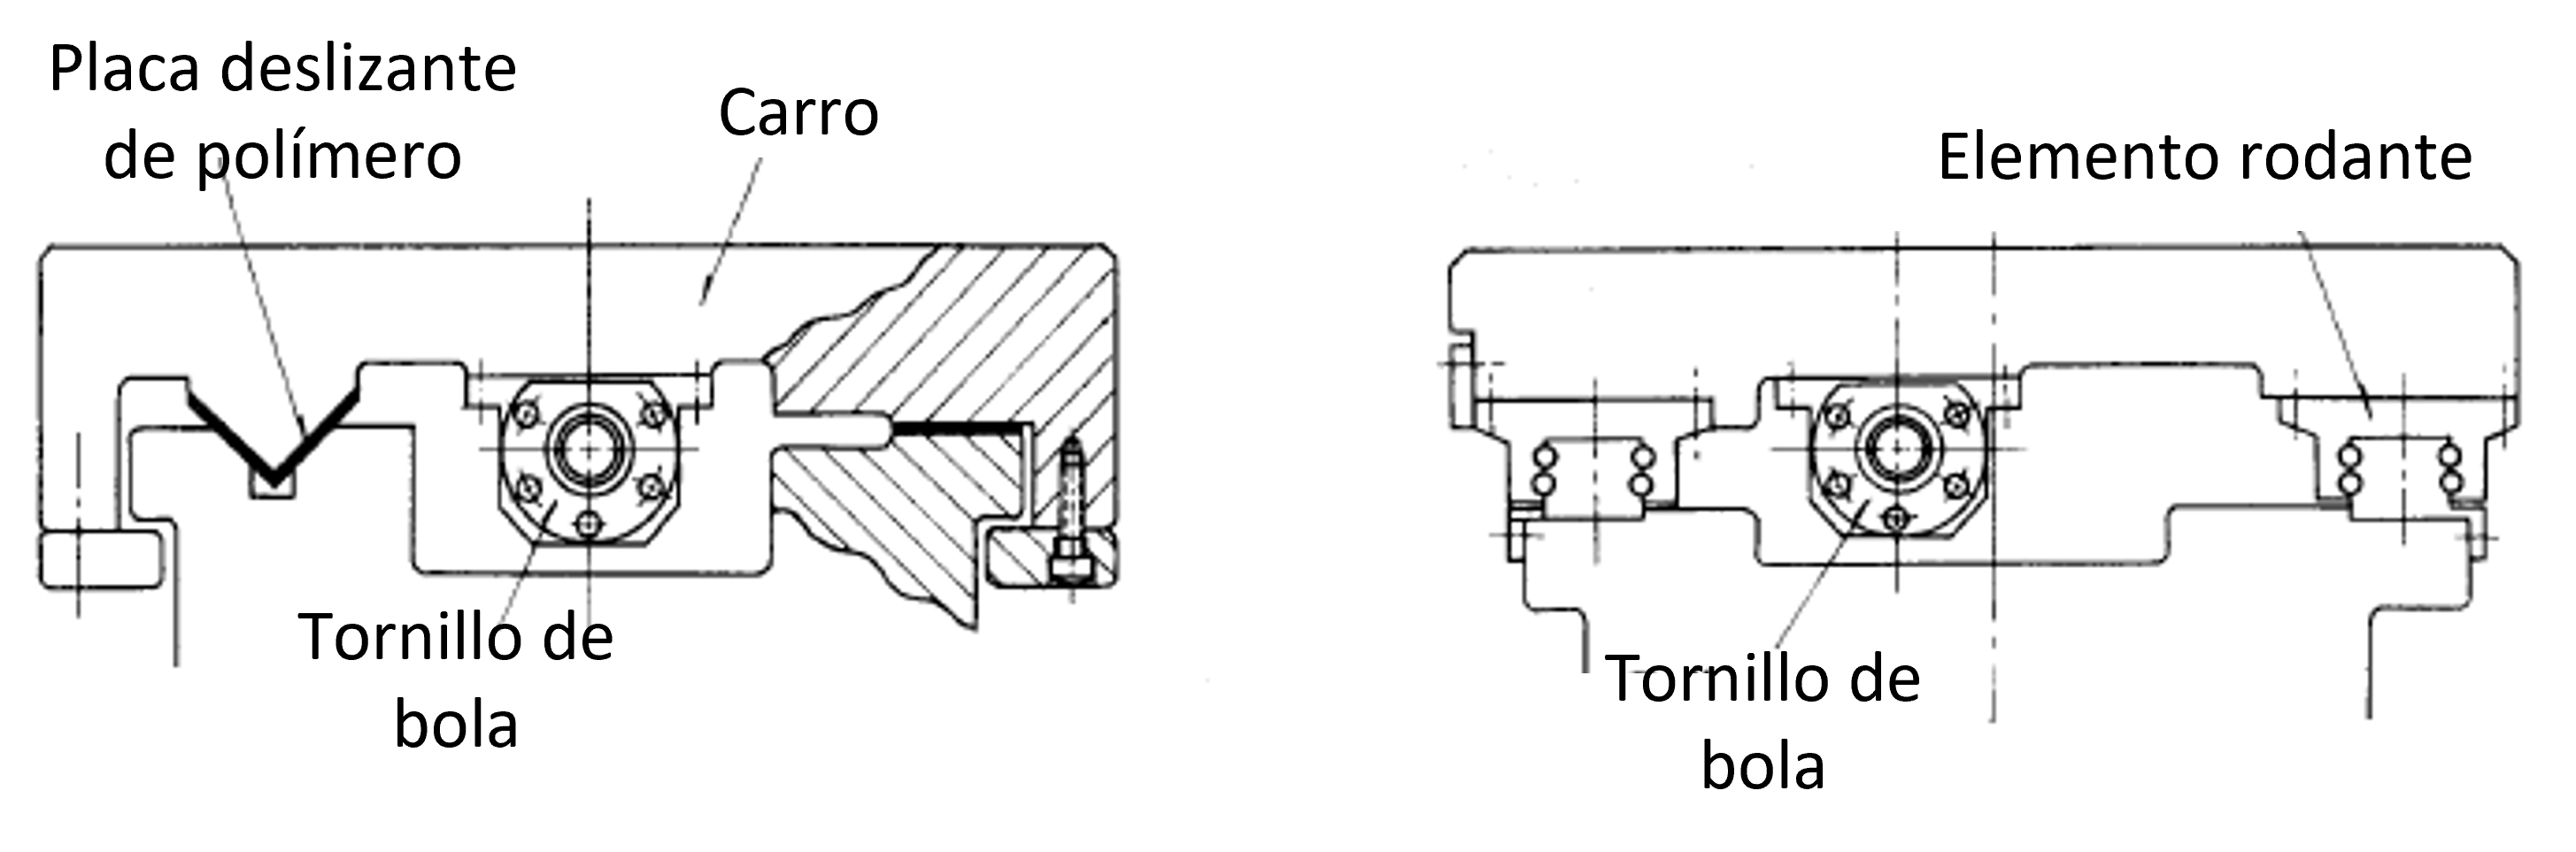
\includegraphics[scale=0.55]{imagenes/rodamientos.png}
    \captionof{figure}{Rodamientos lineales de contacto directo y elementos rodantes \cite{Referencia4}}
    \label{fig:rodamientos}
\end{center}
Los rodamientos lineales pueden ser de contacto directo o con elementos rodantes (bolas o rodillos como los que se muestran en la \emph{figura \ref{fig:rodamientos}}). Los dispositivos de contacto directo son fabricados de un material que genere poca fricción con el material del riel, son más antiguos y más económicos, aún con lubricante los coeficientes de fricción estático y dinámico son altos y difieren mucho entre ellos por lo que no son ideales para aplicaciones de posicionamiento preciso. Por otra lado, los rodamientos lineales con elementos rodantes utilizan un concepto sencillo de reducción de fricción con ayuda de un elemento rotativo, disminuyendo la fuerza para desplazar la masa en comparación con la fuerza que se requiere si la masa estuviera en contacto con toda la superficie de la guía así como se muestra en la \emph{figura \ref{fig:comparativo_friccion}}. Estos rodamientos son elementos mecánicos que contienen múltiples esferas o rodillos internos o externos que giran y cambian de posición dentro de un cilindro interno creando una cadena de movimiento infinita, estos permiten un control más preciso y mejor repetibilidad. La diferencia entre los coeficientes de fricción estáticos y dinámicos son despreciables, esta característica es relevante porque si el coeficiente de fricción estático es considerablemente mayor al dinámico entonces la fuerza que se requiere para empezar a mover el objeto es proporcional y por lo tanto se requiere un cambio de aceleración repentino lo que implica que no se puede alcanzar una velocidad uniforme y se perderá precisión en el posicionamiento, este fenómeno es conocido como \textit{stick-slip} y aunque también está presente en los mecanismos con elementos rodantes su efecto es despreciable \cite{Referencia4}.\\

\begin{center}
    \includegraphics[scale=0.55]{imagenes/comparativo de fricción.png}
    \captionof{figure}{Comparación de fuerza de fricción requerida entre rodamientos de contacto directo y con elementos rodantes \cite{Referencia4}}
    \label{fig:comparativo_friccion}
\end{center}
Existen diferentes tipos de rodamientos lineales con elementos rodantes y se clasifican principalmente por el tipo de elemento rodante, si cuentan con recirculación de elementos, el tipo de guía, el perfil de esta y si es de carrera ranurada o no. En el diagrama de la \emph{figura \ref{fig:diagrama_rodamientos}}, se presentan los \textbf{ejes lineales} como \say{un componente unitario capaz de guiar el deslizamiento de una bola para hacer que su recorrido sea infinito mediante la recirculación de las mismas}. Formalmente se define como un elemento mecánico donde múltiples bolas de acero circulan para permitir una carrera teóricamente infinita, las bolas ruedan por la ranura del riel y cuando llegan a la tapa son forzadas a cambiar de dirección y volver al inicio de su trayectoria por un conducto interno dentro del rodamiento como se muestra en la \emph{figura \ref{fig:eje_lineal}}. \cite{Referencia4}

\begin{center}
    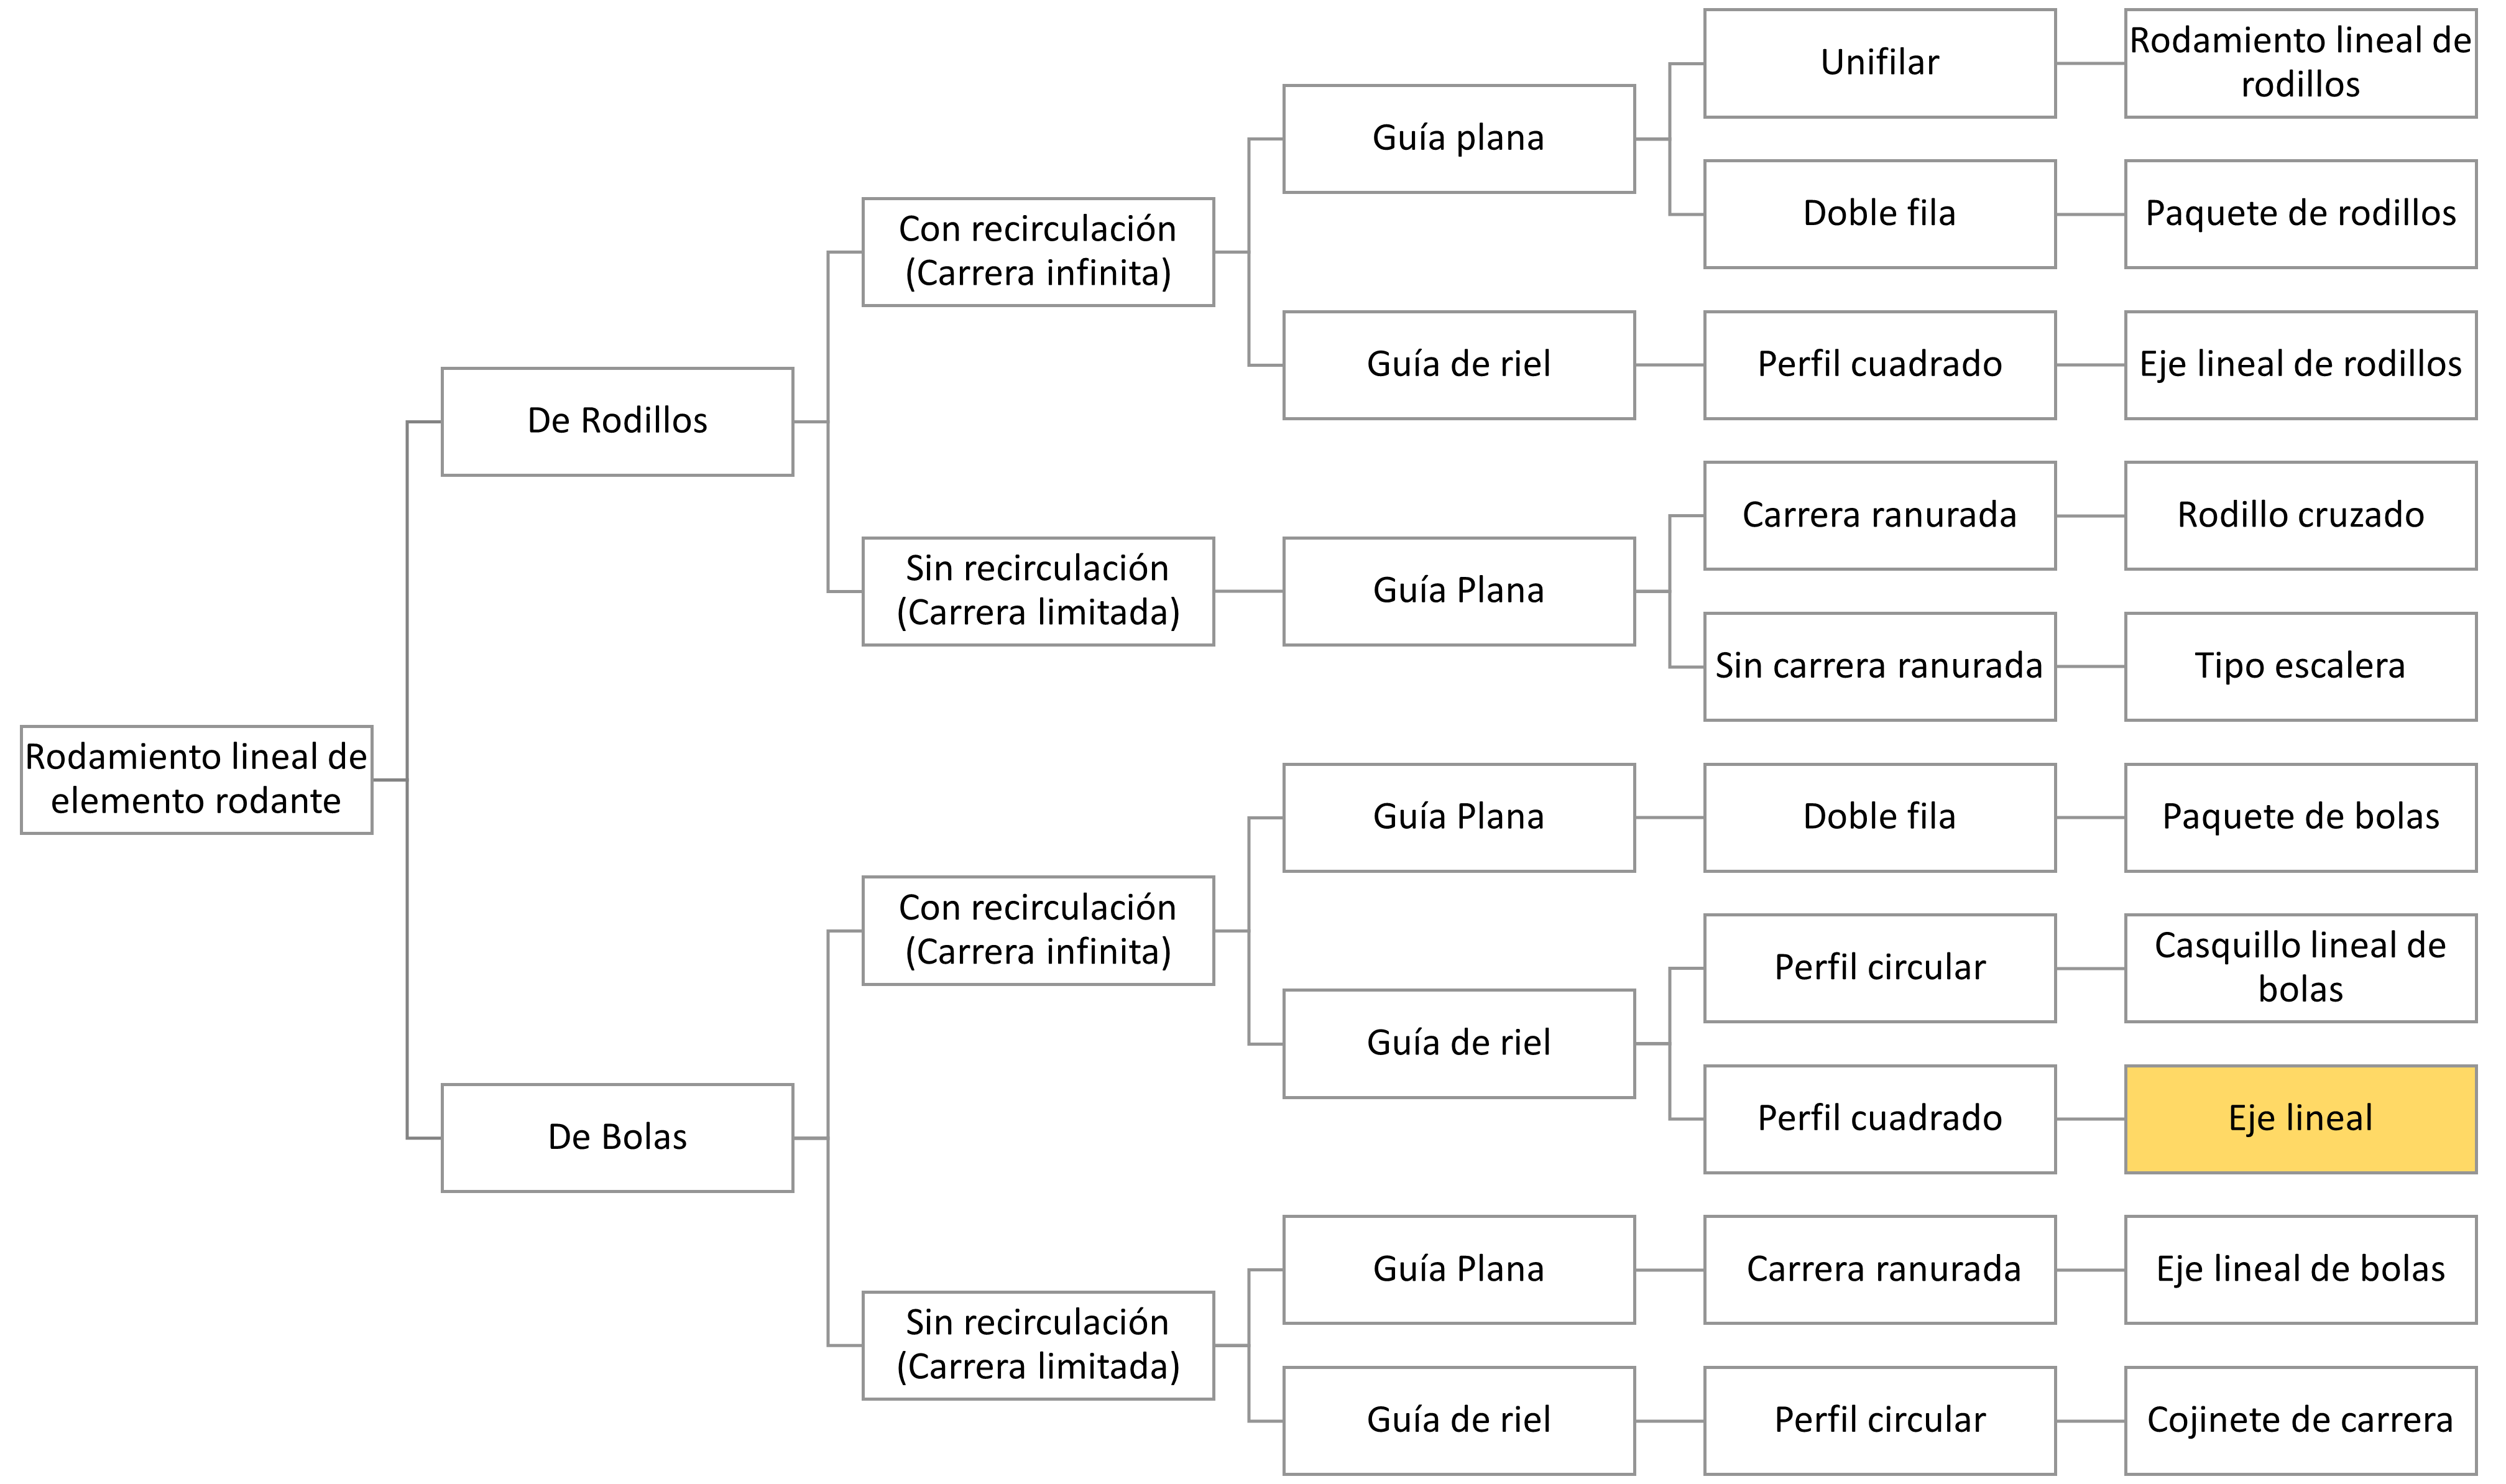
\includegraphics[scale=0.55]{imagenes/diagrama de rodamientos lineales.png}
    \captionof{figure}{Tipos de rodamientos lineales de elemento rodante}
    \label{fig:diagrama_rodamientos}
\end{center}
\begin{center}
    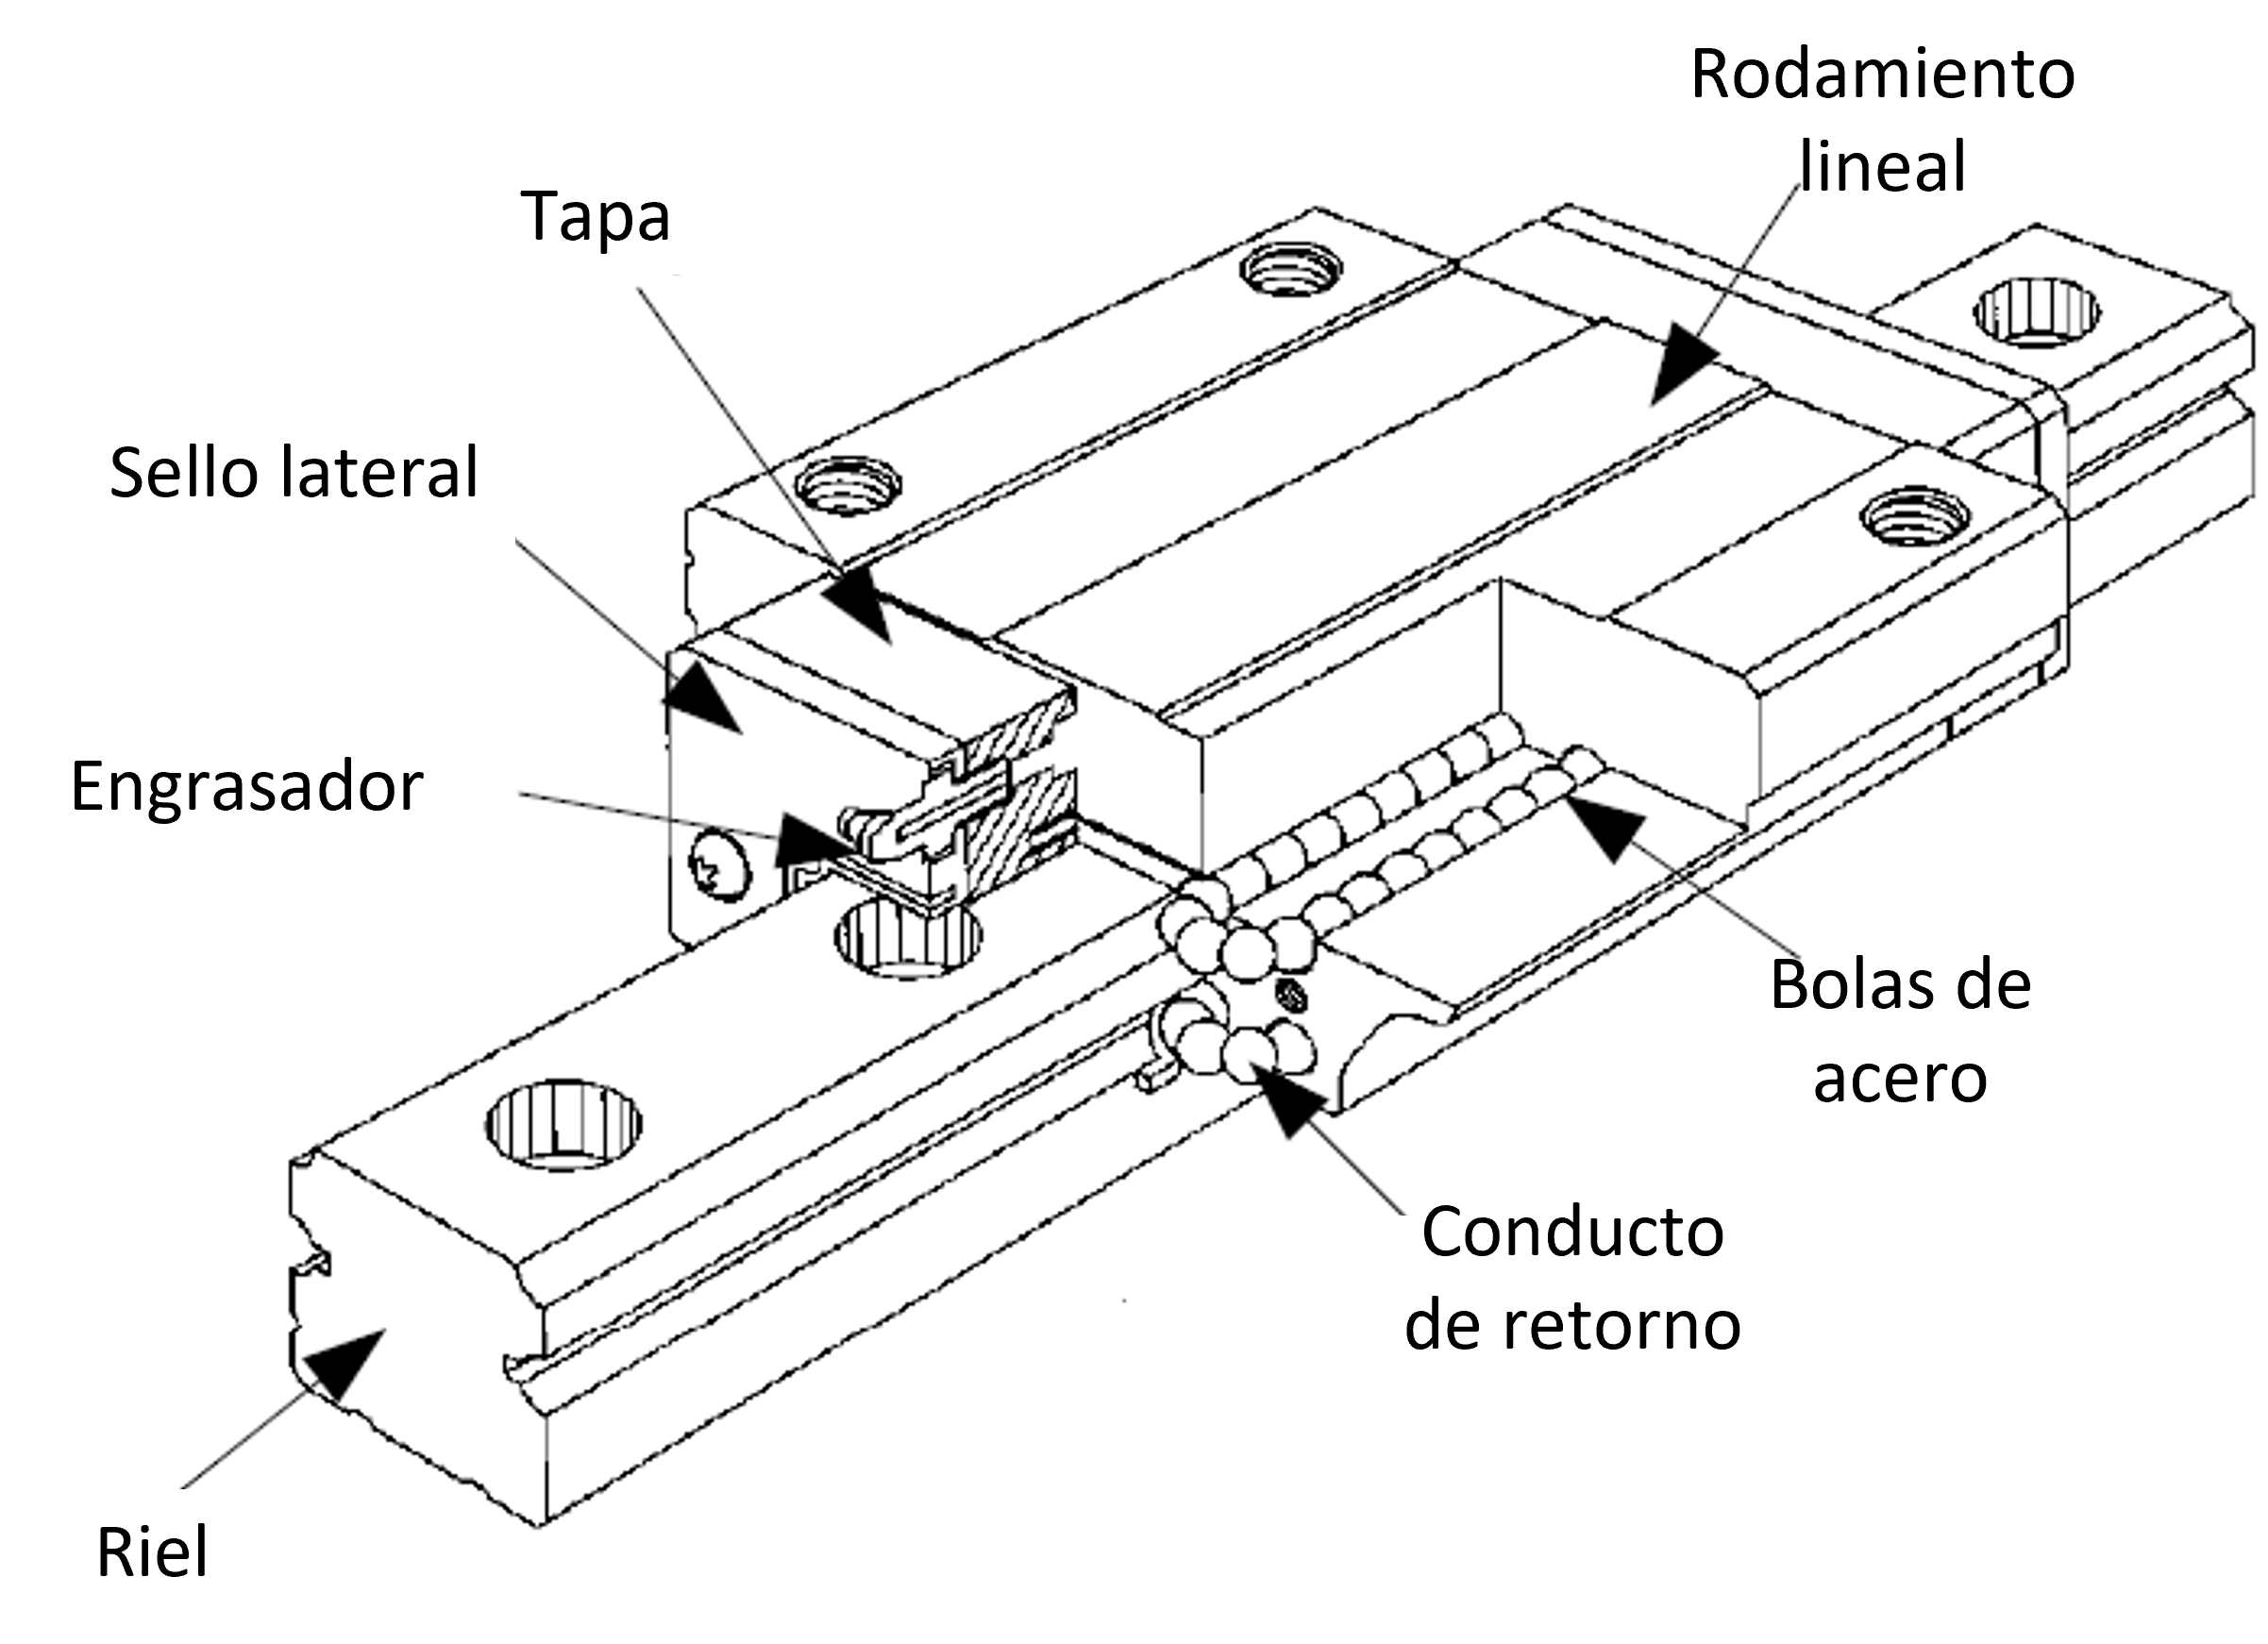
\includegraphics[scale=0.55]{imagenes/Eje_lineal.png}
    \captionof{figure}{Elementos de un eje lineal \cite{Referencia4}}
    \label{fig:eje_lineal}
\end{center}

\subsection{Unidad de transporte robótico}
Una unidad de transporte robótico (UTR) consiste de un robot articulado (típicamente de 4 a 6 grados de libertad) con capacidad de carga media o baja montado sobre una vía o eje lineal auxiliar que se desplaza en la misma dirección que el flujo de trabajo de la línea de producción (véase \emph{figura \ref{fig:utr}}). Cualquier actuador lineal puede utilizarse para estas aplicaciones (bandas, cremallera y piñón, motor lineal, tornillo sin fin).\\
\begin{center}
    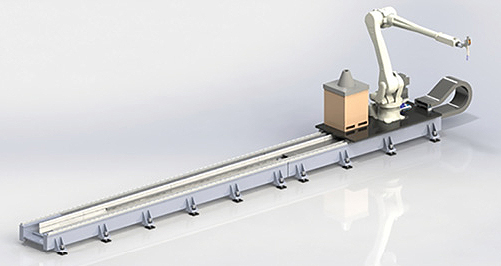
\includegraphics[scale=0.55]{imagenes/Kawasaki-transport-unit-RTU.jpg}
    \captionof{figure}{Unidad de transporte robótico para un robot Kawasaki \cite{Referencia5}}
    \label{fig:utr}
\end{center}
Los 2 criterios determinantes en el diseño de unidades de transporte robótico son la velocidad y la precisión, para establecer el factor principal entre estos 2 criterios se debe tomar en cuenta aplicación de la UTR, por ejemplo, si se necesita que el robot recorra varios metros para carga y descarga de material la velocidad será el factor principal, pero si por el contrario. Dentro del contexto de UTRs una velocidad de $3m/s$ se considera relativamente rápida (considerando que estas unidades pueden llegar a cargar cientos de kilogramos). Otro factor importante es durabilidad y bajo mantenimiento para estas unidades ya que el tiempo que estén fuera de servicio afecta múltiples áreas de una celda de manufactura. \cite{Referencia5}.\\
El reto de ingeniería más complejo de una UTR es la sincronización con el robot articulado que transporta, existen 2 opciones de control, asíncrona y síncrona, en el primer caso, el eje lineal y el robot articulado están desacoplados y el movimiento del eje lineal está condicionado por los ciclos de trabajo del robot por lo que el control de estos sistemas es más sencillo que en el segundo caso donde se debe considerar el sistema como un 7mo grado de libertad lo que permitiría realizar trayectorias más complejas pero la planeación de trayectorias también se complica, en la industria típicamente se usan herramientas de software y hardware que permiten la programación tanto del robot articulado como del UTR, y mediante el \emph{teach pendant} se programan las posiciones deseadas y las configuraciones del efector final.\\

\subsection{Robotic Operating System}
A pesar de que en su nombre se menciona \say{sistema operativo} realmente ROS es un \emph{middleware} para aplicaciones robóticas. Sin embargo, proporciona todos los servicios que se pueden esperar de un sistema operativo como administración de hardware y periféricos, comunicación entre procesos y manejo de paquetes. ROS es un compendio de herramientas y librerías que facilitan la programación de sistemas robóticos, que al ejecutarse corre una red de procesos \say{peer-to-peer} dentro de un grafo computacional con distintos elementos. Los elementos básicos dentro de este grafo son \emph{nodos, maestros, parámetros del servidor, mensajes, servicios, temas, y bolsas}. El maestro almacena información sobre los temas y servicios registrados para otros nodos. Estos nodos se reportan con el maestro para recibir información de otros nodos y realizar las conexiones adecuadas, una vez establecida esta conexión los nodos se pueden comunicar de forma directa sin necesidad de recurrir al maestro, de igual forma cuando se cambia la información de registro de algún nodo el maestro se comunica con los nodos correspondientes para crear o destruir conexiones de forma dinámica aún con los nodos en ejecución. En ROS el protocolo de comunicación que se usa es llamado TCPROS que en realidad es un estándar de sockets TCP/IP, los nodos se comunican publicando o al suscribirse a cierto \say{tema} como en la \emph{figura \ref{fig:ros_topic}} \cite{Referencia6}.
\begin{center}
    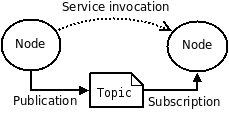
\includegraphics[scale=0.7]{imagenes/ros_topic.png}
    \captionof{figure}{Comunicación entre nodos de ROS \cite{Referencia6}}
    \label{fig:ros_topic}
\end{center}
